

\capitulo{5}{Aspectos relevantes del desarrollo del proyecto}

\begin{comment}
Este apartado pretende recoger los aspectos más interesantes del desarrollo del proyecto, comentados por los autores del mismo.
Debe incluir desde la exposición del ciclo de vida utilizado, hasta los detalles de mayor relevancia de las fases de análisis, diseño e implementación.
Se busca que no sea una mera operación de copiar y pegar diagramas y extractos del código fuente, sino que realmente se justifiquen los caminos de solución que se han tomado, especialmente aquellos que no sean triviales.
Puede ser el lugar más adecuado para documentar los aspectos más interesantes del diseño y de la implementación, con un mayor hincapié en aspectos tales como el tipo de arquitectura elegido, los índices de las tablas de la base de datos, normalización y desnormalización, distribución en ficheros3, reglas de negocio dentro de las bases de datos (EDVHV GH GDWRV DFWLYDV), aspectos de desarrollo relacionados con el WWW...
Este apartado, debe convertirse en el resumen de la experiencia práctica del proyecto, y por sí mismo justifica que la memoria se convierta en un documento útil, fuente de referencia para los autores, los tutores y futuros alumnos.
\end{comment}

En el siguiente apartado se realizará un explicación de los aspectos más relevantes del proyecto. De esta manera, se explicarán los problemas surgidos y las solución aplicada para su resolución.

\section{Recogida de datos}
La obtención de los datos necesarios para el posterior análisis, se realizó a través de la organización europea \emph{Copernicus}. Esta cuenta con una serie de datos recopilados por satélites de todo el mundo.

Para la descarga de estos datos, se encontraban disponibles dos alternativas. Por un lado, podían ser descargados a través de un servidor FTP y por el otro, había disponible una API de reciente lanzamiento.

En un principio se priorizó la opción de la descarga a través de la API ya que podían descargarse los datos ya tratados reduciendo el trabajo previo al análisis. Finalmente se descartó esta idea por la lentitud de respuesta del servicio, así como diferentes errores que se producían, haciendo que la descarga de la totalidad de los datos no estuviese asegurada. Por este motivo se descargaron los datos a través del servidor FTP y posteriormente, eran tratados eliminando las variables y zonas geográficas que no eran necesarias.

Si se desea acceder a la plataforma de \emph{Copernicus}, se proporciona la cuenta con que se ha utilizado para la realización del proyecto:
\begin{itemize}
	\item \textbf{Usuario:} psantidriantuda
	\item \textbf{Contraseña:} UBUinformatic@2020
	\item \textbf{Web:} \href{https://resources.marine.copernicus.eu/?option=com_csw&task=results}{https://resources.marine.copernicus.eu/?option=com\_csw\&task=results}
\end{itemize}


\section{Ejecución remota}
Para la ejecución de los scripts utilizados para la descarga de los datos, la ejecución del modelo y la realización de las diferentes pruebas, se ha utilizado un equipo de cómputo de la Universidad mediante una conexión ssh y una VPN. El uso de esta máquina fue necesario por el gran tamaño de los datos descargados en un primer momento, así como para el entrenamiento de los modelos, ya que fueron tareas con largos tiempos de ejecución y me permitía no tener mi equipo encendido durante tanto tiempo.Todo esto ha hecho que surjan diferentes problemas.

En primer lugar no se disponía de permisos de administrador para instalar las diferentes bibliotecas necesarias. Esto se solucionó mediante la instalación de la distribución local Anaconda que nos permite ser instalada para un único usuario. Con esto, se creó un entorno virtual en el que poder instalar todas las bibliotecas necesarias.

\subsection{tmux}
Como se ha explicado anteriormente al hablar de tmux (\ref{tmux}), se ha tenido problemas a la hora de ejecutar los diferentes scripts en el equipo de cómputo.

Para la ejecución de las diferentes pruebas, se utilizado la conexión ssh lanzado un proceso de Jupyter Notebook sin interfaz gráfica mediante el comando \verb|jupyter notebook --no-browser|. Posteriormente, se conecta el puerto en que se ejecuta jupyter en la máquina de cómputo, con un puerto en un equipo personal y de esta manera, trabajar como si la ejecución de los \emph{Notebooks} se realizase en local.

%Este servidor se inicializa por defecto en el puerto local 8888 por lo que se utiliza el comando \emph{"ssh -p 22 -N -f -L localhost:9006:localhost:8888 pst0004@10.168.168.11"} para conectar este puerto del equipo de cómputo con un puerto (en este caso el 9006) de un equipo personal.

Existían casos en los que la conexión ssh se cerraba o se caía la conexión VPN, por lo que se perdía el proceso de ejecución o los últimos cambios realizados en los notebooks no se guardaban. Para eso se utilizó la herramienta tmux permitiendo, que aunque la conexión se perdiera, los procesos en segundo plano no se perdían y así poder continuar con el trabajo.

\section{Preparación de los datos}\textsl{}
Tras haber descargado los datos oceánicos, disponemos de dos fuentes de datos. Por una lado, el estado de los océanos en las diferentes fechas y coordenadas, y por otro, un registro de avistamientos de medusas.

Los datos oceánicos están agrupados por cuadrantes separados cada \num{0,0833}  grados (1/12). Por esto se redondearon las coordenadas de los avistamientos para coincidir con estos pasos. 

A continuación se enlazan en un solo \emph{DataFrame} los avistamientos con la variables oceánicas recogidas de ese cuadrante y en la fecha del avistamiento quedando la siguiente estructura de datos como la que encontramos en la figura \ref{dataframe_datos}.

Un \emph{DataFrame} se trata de una estructura de datos de dos dimensiones similar a una tabla de una hoja de cálculo, en la que podemos guardar datos de diferentes tipos ordenados en filas y columnas.

\begin{figure}%[!h]
	\centering
	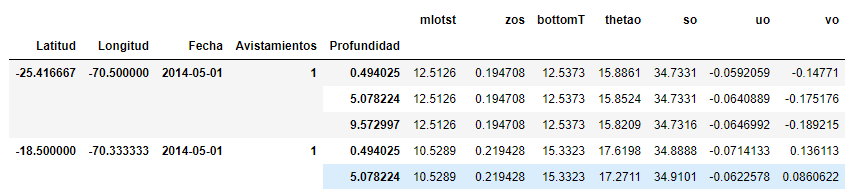
\includegraphics[width=1\textwidth]{estructura_datos.png}
	\caption[Estructura de datos resultante.]{Estructura de datos resultante.}\label{dataframe_datos}
\end{figure}


Esta estructura inicial, contiene poca información, pues no se puede predecir con exactitud la aparición de medusas observando únicamente el cuadrante más próximo a las playas. Por ello se añadieron más lecturas de los cuadrantes adyacentes mar adentro. Estos nuevos cuadrantes fueron incluidos a la estructura inicial modificando el nombre con una etiqueta al final de las mismas para poder identificarlos. El resultado de como se organizan estas etiquetas se puede observar en la figura \ref{croquis_cuadrantes}.

\begin{figure}%[!h]
	\centering
	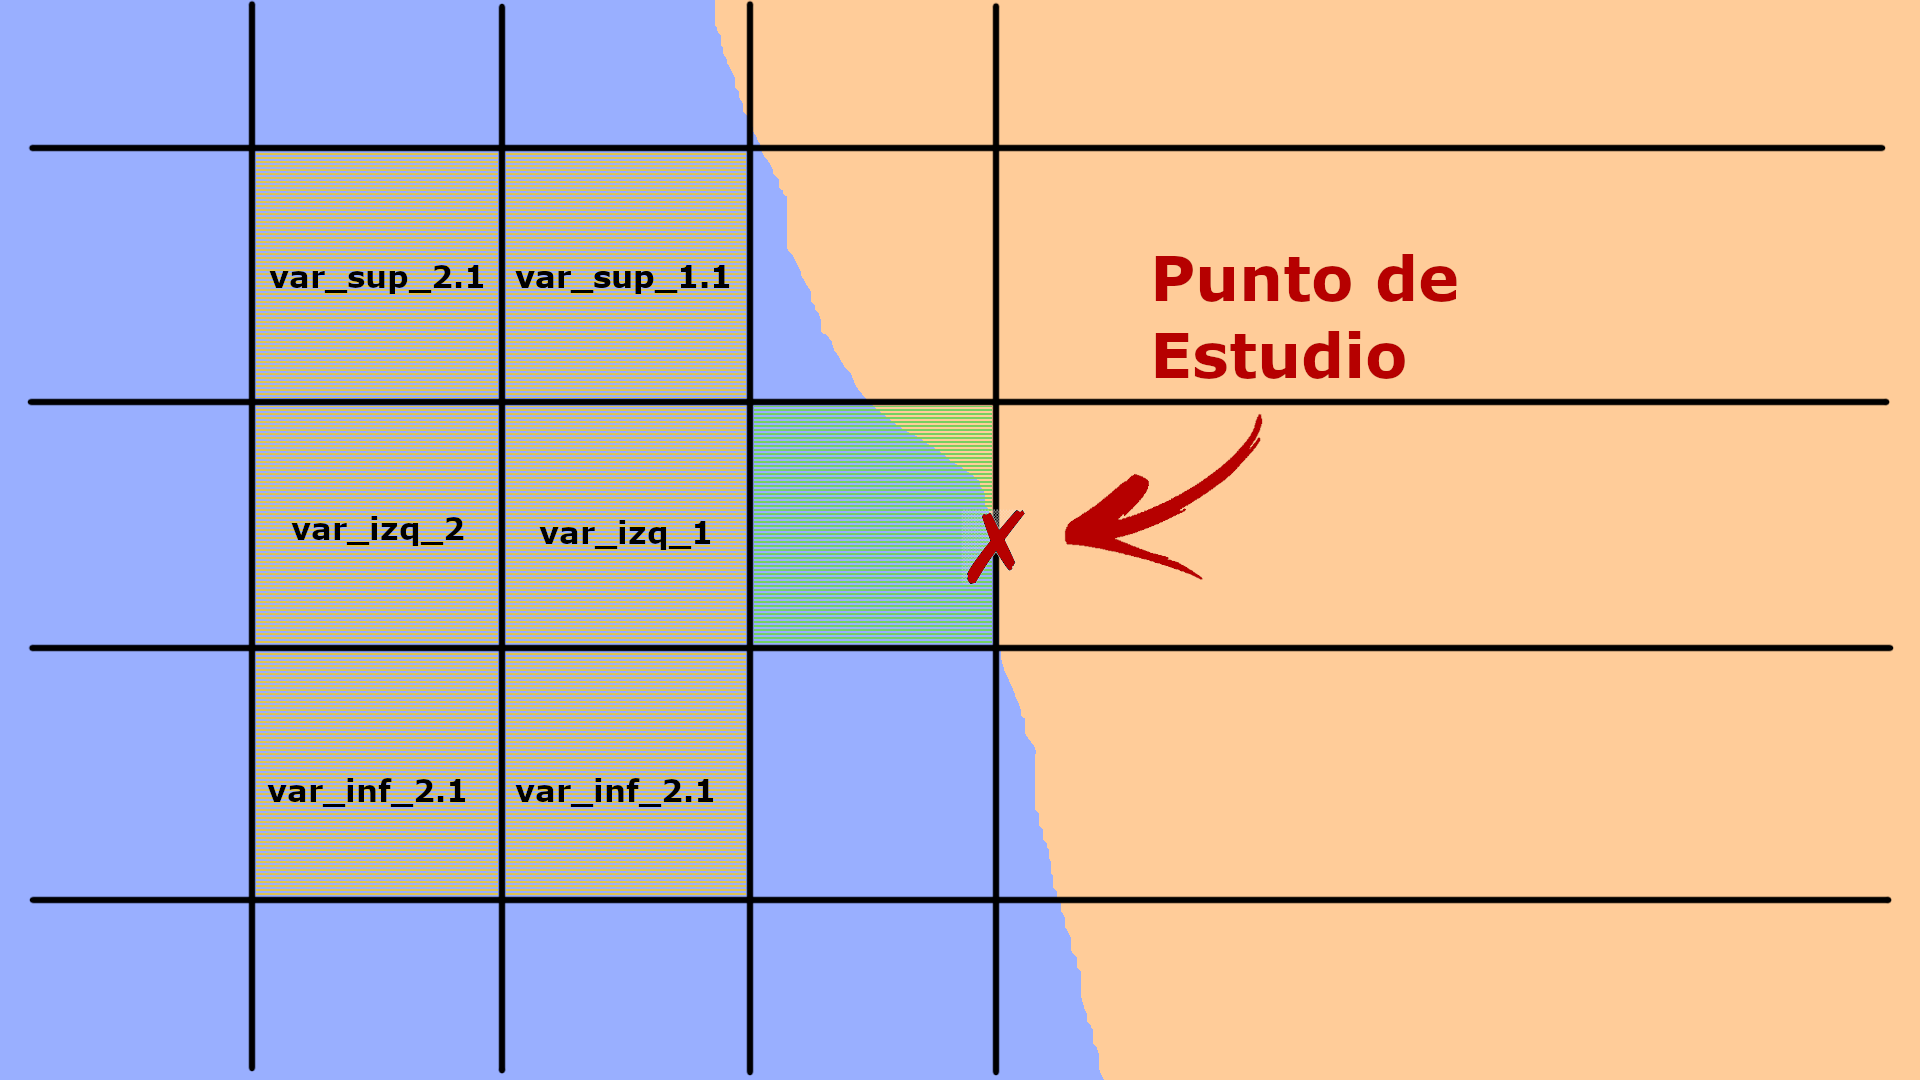
\includegraphics[width=1\textwidth]{croquis_cuadrantes.png}
	\caption[Croquis de referencia sobre los cuadrantes y el nombre de las variables asociadas.]{Croquis de referencia sobre los cuadrantes y el nombre de las variables asociadas.}\label{croquis_cuadrantes}
\end{figure}

Tras unir todos los cuadrantes nos encontramos que ciertas celdas no contenían información. Esto se debe principalmente por dos causas: Las profundidades se toman a 0, 5 y 10 metros, esto hace que en los cuadrantes más cercanos a las costas existiesen zonas con una profundidad inferior. También debido a la forma de la línea de costa, existen zonas en las que ya sean cuadrantes inferiores o superiores, están situados tierra adentro.

La solución que se buscó a este problema, fue la de utilizar los datos del cuadrante más cercano por la izquierda que tenga información válida.

\section{Despliegue de la aplicación web}
Al tratarse se una aplicación web, un aspecto importante es el despliegue de la misma en un servidor al que poder acceder desde cualquier lugar. Como se ha mencionado en la sección de herramientas (\ref{HerokuHerrramientas}), se ha utilizado la aplicación \emph{Heroku}.

Esta nos ofrece hosting gratuito, además de desplegarse automáticamente cada vez de que se realiza un \emph{push} en el repositorio, si este está asociado a la cuenta de heroku. Por este motivo, se tuvo que realizar un segundo repositorio en Github en el que incluir únicamente la parte de la aplicación web, ya que para poder realizar el autodespliegue los archivos deben estar en el directorio raíz de nuestro repositorio.

Se añadió una referencia desde el repositorio principal a este segundo ya que \emph{Git} lo permite, además de incluir el enlace también en el archivo README. 

El repositorio se encuentra en \url{https://github.com/psnti/WebJellyfishForecast}.


